\documentclass[12pt, a4papre]{article}
\usepackage[catalan]{babel}
\usepackage[unicode]{hyperref}
\usepackage[dvipsnames]{xcolor}
\usepackage{amsmath}
\usepackage{amssymb}
\usepackage{amsthm}
\usepackage{xifthen}
\usepackage{siunitx}
\usepackage{xcolor}
\usepackage{float}
\usepackage{listings}
\usepackage{setspace}
\usepackage{graphicx}
\usepackage{tikz,lipsum,lmodern}
\usepackage[most]{tcolorbox}
\usepackage{multicol}
\usepackage{fancyvrb}
\usepackage{circuitikz}
\usepackage{indentfirst}
\usepackage{verbatimbox}
\usepackage{verbatim}
\usepackage[utf8]{inputenc}
\definecolor{mygreen}{RGB}{28,172,0} % color values Red, Green, Blue
\definecolor{mylilas}{RGB}{170,55,241}
\graphicspath{ {./Images/} }

\newcommand{\norm}[1]{\lvert #1 \rvert}

\hypersetup{
    colorlinks = true,
    linkcolor = blue
}

\author{Daniel Vilardell}
\title{Memoria practica 1 ONELE}
\date{}

\begin{document}
	\maketitle
	\textbf{Ejercicio 1:} Al laboratori vam prendre les següents mesures:
	
	\begin{center}
		\begin{tabular}{ ||c|c|| } 
			\hline
			& Potencia\\ 
			\hline
			$P_{ref}$ & 2.62\\ 
			$P_{vidrio}$ & 2.33\\ 
			$P_{pyrex}$ & 2.35\\ 
			\hline
		\end{tabular}
	\end{center}
	
	Per tant obtenim que 
	
	\[
		T_{pyrex} = \frac{2.35}{2.62} = 0.896 \quad T_{pyrex} = \frac{2.33}{2.62} = 0.889
	\]
	
	Veiem que els valors de transmitivitat son molt propers al teoric  ($T = 0.917$).\\
	
	\textbf{Ejercicio 2:} Els valors de potencia mesurats amb el laser i el pyrex en contes del led son els seguents. Es van fer varies mesures per a poguer agafar la mitja
	
	\begin{center}
		\begin{tabular}{ ||c|c|| } 
			\hline
			& Potencia\\ 
			\hline
			$P_{ref}$ & 2.02\\ 
			$P_1$ & 1.90\\ 
			$P_2$ & 1.82\\ 
			$P_3$ & 1.88\\ 
			$P_4$ & 1.72\\ 
			\hline
		\end{tabular}
	\end{center}
	
	Per tant tenim que 
	
	\[
		\frac{1.90+1.82+1.88+1.72}{4\cdot 2.02} = 0.923
	\]
	
	Veiem que el resultat es proper al teoric pero les mostres son bastant irregulars. El LED es menys coeerent que el laser temporalment.
	
	Busquem ara $T_{max}$ i $T_{min}$.
	
	\begin{center}
		\begin{tabular}{ ||c|c|| } 
			\hline
			& Potencia\\ 
			\hline
			$P_{ref}$ & 8.46\\ 
			$P_{min}$ & 6.93\\ 
			$P_{max}$ & 7.48\\ 
			\hline
		\end{tabular}
	\end{center}
	
	I d'aquí obtenim que 
	
	\[
		T_{min} = \frac{6.93}{8.46} = 0.819 \quad T_{max} = \frac{7.48}{8.46} = 0.884
	\]
	
	Rarament dona mes petit que el teoric o el trobat al exercici 1. S'hauria de tornar a fer les mesures per a assegurar que son correctes.\\
	
	\textbf{Exercici 3:} Tenim que els medis tenen permeavilitats $n_1 = n_4 = 1$, $n_2 = 4.1$, $n_3 = 1.52$. Per tant d'aquí podem calcular $\tau_{21}, \tau_{32}, \tau_{43}$.
	
	\[
		\tau_{21}= 1+\rho_{21}= \frac{2n_2}{n_2+n_1} = 1.61 \quad \tau_{32}=1+\rho_{32}=\frac{2n_3}{n_3+n_2} = 0.54 
	\]
	
	\[
		\tau_{43}=\frac{2n_4}{n_4+n_3} = 0.79
	\]
	
	\[
		T = \frac{|\tau_{21}|^2|\tau_{32}|^2|\tau_{43}|^2}{|1+\rho_{21}\rho_{32}e^{-2jkn_2d}|^2}
	\]		
	
	Ara que tenim $T$ en funció de la distancia ho grafiquem a matlab i despres busquem la T per les tres lamines estudiades al laboratori.
	
	\begin{figure}[H]
		\begin{center}
		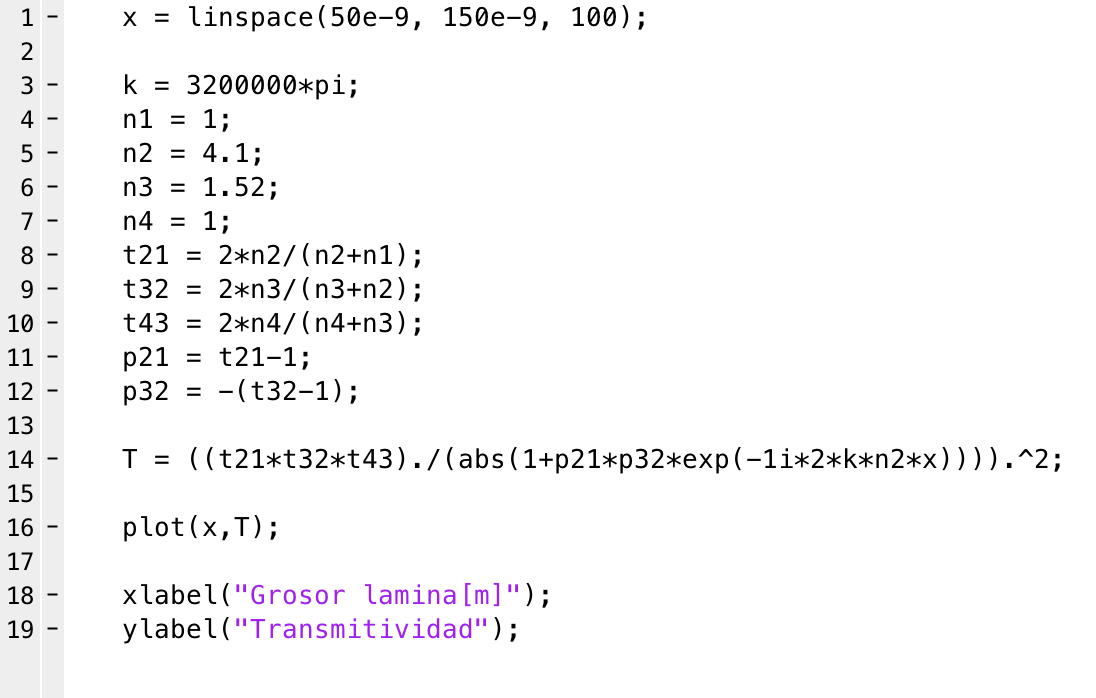
\includegraphics[width=110mm]{pr2_2.png}
		\caption{Codi matlab usat per a generar la grafica}
		\end{center}
	\end{figure}
	
	\begin{figure}[H]
		\begin{center}
		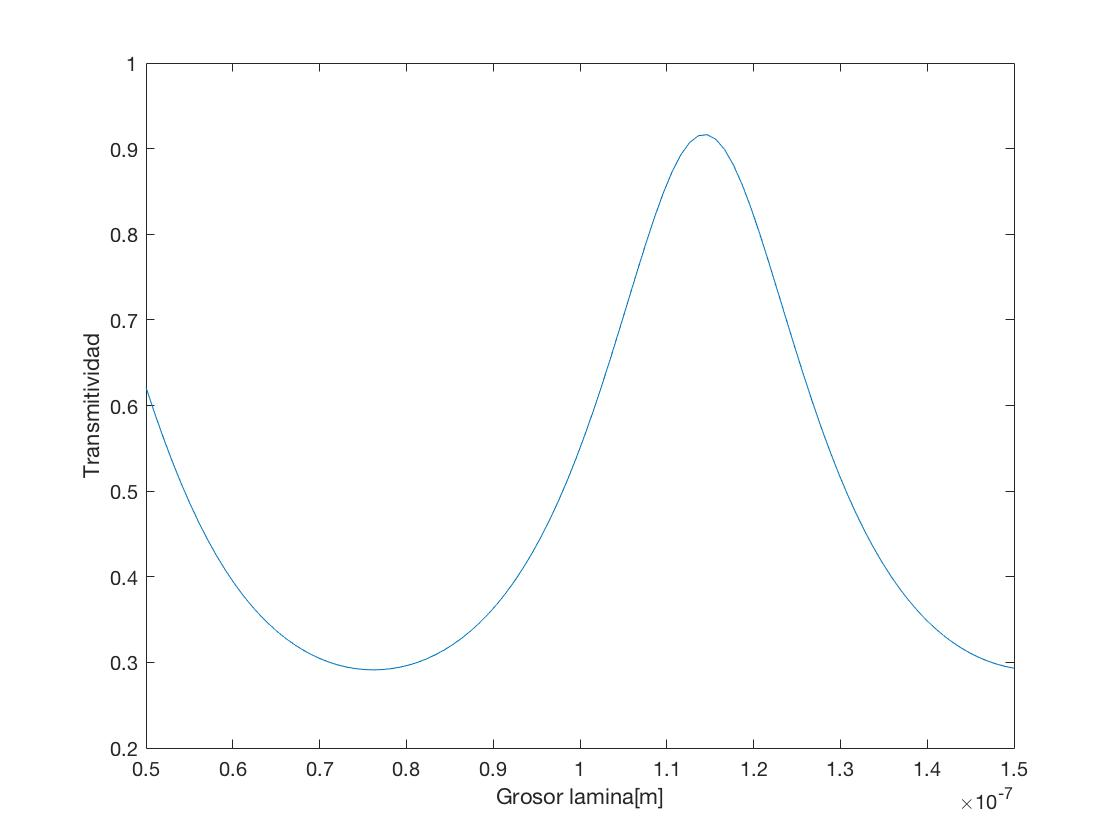
\includegraphics[width=110mm]{pr2_1.jpg}
		\caption{Transmitividad en funcion del grosor de la lamina}
		\end{center}
	\end{figure}
	
	D'aquí, tenint en conte que $P_{ref} = 1.66$ podem obtenir a partir de les dades experimentals que que les lamines tenen transmitivitat
	
	\[
		T_{08} = 0.6 \quad T_{12} = 1.1 \quad T_{16} = 0.49
	\]
	
	i per tant podem veure a la grafica que els grossors son de 
	
	\[
		G_{08} = 105nm\text{ o }123nm \quad G_{12} = 115nm \quad G_{16} = 51nm\text{, }100nm\text{ o }130nm
	\]
	
	
	
\end{document}










